\documentclass{article}

% Language setting
% Replace `english' with e.g. `spanish' to change the document language
\usepackage[english]{babel}

% Set page size and margins
% Replace `letterpaper' with `a4paper' for UK/EU standard size
\usepackage[letterpaper,top=2cm,bottom=2cm,left=3cm,right=3cm,marginparwidth=1.75cm]{geometry}

% Useful packages
\usepackage{amsmath}
\usepackage{graphicx}
\usepackage[colorlinks=true, allcolors=blue]{hyperref}
\usepackage{listings}

\usepackage[style=authoryear-ibid,backend=biber]{biblatex}

\usepackage{xcolor}

\usepackage{csquotes}% Recommended
\addbibresource{projectreport.bib}% Syntax for version >= 1.2

\definecolor{codegreen}{rgb}{0,0.6,0}
\definecolor{codegray}{rgb}{0.5,0.5,0.5}
\definecolor{codepurple}{rgb}{0.58,0,0.82}
\definecolor{backcolour}{rgb}{0.95,0.95,0.92}

\lstdefinestyle{pythonstyle}{
    backgroundcolor=\color{backcolour},   
    commentstyle=\color{codegreen},
    keywordstyle=\color{magenta},
    numberstyle=\tiny\color{codegray},
    stringstyle=\color{codepurple},
    basicstyle=\ttfamily\footnotesize,
    breakatwhitespace=false,         
    breaklines=true,                 
    captionpos=b,                    
    keepspaces=true,                 
    numbers=left,                    
    numbersep=5pt,                  
    showspaces=false,                
    showstringspaces=false,
    showtabs=false,                  
    tabsize=2
}

\lstset{style=pythonstyle}

\begin{document}

\begin{titlepage}
    \begin{center}
        \vspace*{1cm}
        \LARGE\textbf{CCT College Dublin}\\
        \vspace{0.5cm}
        \Large Assessment Cover Page\\
        \hrulefill\\
        \vspace{1cm}
        \begin{tabular}{|l|p{7cm}|}
        
        \hline
        Module Title:& Strategy Thinking \\
        \hline
        Assessment Title:& Project Report\\
        \hline
        Lecturer Name:& James Garza\\
        \hline
        Student Full Name:& Giulio Calef, Kevin Byrne and Victor Ferreira Silva \\
        \hline
        Student Number:& sba22314, sba22264, 2021324 \\
        \hline
        Assessment Due Date:& 7th May 2023\\
        \hline
        Date of Submission:& 7th May 2023\\
        \hline
        \end{tabular}
        
        \vspace{1cm}
        \Large Declaration\\
        \vspace{0.5cm}
        \normalsize By submitting this assessment, I confirm that I have read the CCT policy on Academic Misconduct and understand the implications of submitting work that is not my own or does not appropriately reference material taken from a third party or other source. I declare it to be my own work and that all material from third parties has been appropriately referenced. I further confirm that this work has not previously been submitted for assessment by myself or someone else in CCT College Dublin or any other higher education institution.\\
    \end{center}
\end{titlepage}


\begin{titlepage}
   \begin{center}
       \vspace*{1cm}

       \textbf{Detecting and Predicting Severe Slugging in Petrobras 3W Data Set}

       \vspace{0.5cm}
        Strategic Thinking Capstone Project
            
       \vspace{1.5cm}

       \textbf{Giulio Calef} \\
       \textbf{Kevin Byrne} \\
       \textbf{Victor Ferreira Silva} \\

       \vfill
            
       Strategic Thinking Capstone Project
            
       \vspace{0.8cm}
     
       % \includegraphics[width=0.4\textwidth]{university}
            
       Higher Diploma in Science in Artificial Intelligence Applications\\
       CCT College Dublin\\
       Ireland\\
       May 2023
            
   \end{center}
\end{titlepage}

\title{Detecting and Predicting Severe Slugging in Petrobras 3W Data Set}

\author{Giulio Calef, Kevin Byrne, Victor Ferreira Silva}
\tableofcontents

\maketitle

\section{Abstract}
Operational and environmental safety, productivity, quality are general key objectives in many industries, and in the oil and gas industry this concerns are not only crucial, but they also pose as an immense daily challenge given the complexity of their operations. This project aims to detect the presence or point the absence of Severe Slugging in offshore oil well production lines using machine learning techniques. The real instances of 3W Data Set from Petrobras were used to train and test the classification models here described, and all iterations in this project followed the CRISP-DM methodology, considered the realistic aspects of 3W Data Set, observed the strongest correlations between some features and the target and performed an extensive hyperparametrisation tuning for all models before the evaluation stage. Lastly, all these models were evaluated according their accuracy, precision, and recall, and as a result, two classifiers - Random Forest Classifier and Decision Tree Classifier - demonstrated remarkable results in comparison to other three models (namely, Artificial Neural Networks, k-Neighbours Classifier and LinearSVC). The project contributed to the successful development of classification models capable to detect Severe Slugging, therefore helping offshore oil operations to succeed in mitigating safety risks, reducing operational costs, and improving production efficiency. 

\section{Introduction}

Generally, the oil industry has been increasingly adopting automated controls and monitoring processes \parencite{venkatasubramanian_rengaswamy_yin_kavuri_2003} to comply with the increasingly higher standards in their operations. Such standards not only require more productive operations, but safer processes and more energy-efficient methods to achieve greater quality \parencite{jounela_2007}. 

All this increasing investment also aims to build processes that can timely detect faults or anomalous systematic behaviours which can affect the normal state of the operations, ultimately causing undesirable events in production line. Such events, for example, were responsible for most of the production loss at Petrobras Operational Unit located in the Brazilian state of Espírito Santo (UO-ES) in 2016 \parencite{revvargas2019}, which was around 1.5 million barrels, that is, US\$75.7 million - the average value of the barrel was approximately US\$50 at the time.

After this, tn 2017 Petróleo Brasileiro S.A., the Brazilian oil company known as Petrobras, launched a project named \emph{“Monitoramento de Alarmes Especialistas"} (“Expert Alarm Monitoring" - MAE) to improve its abnormal event management (AEM) in oil and gas wells and  to complement their monitoring processes at the time. The project MAE aimed to create a new automated AEM to detect and classify 8 specific \emph{undesirable events} in offshore naturally flowing wells.  

Among these above-mentioned undesirable events, there is an event known as \emph{Severe Slugging}, which can be defined as a critical flow assurance issue, commonly observed in offshore pipeline-riser systems, documented for the first time by \textcite{yocum_1973}. Some of the consequences of this issue include flooding of downstream production facilities and an overall decrease in productivity. According \textcite{revvargas2019} depending on the frequency it occurs and intensity, this event may even damage the equipment in the well, although specific operational actions can be taken to mitigate this issue since it is detected.

Considering that, Petrobras has developed the 3W Project, which is a project built upon the 3W Data Set and the 3W Took Kit. The former is a database defined by \textcite{revvargas2019} and it contains instances from three different sources and contains data on undesirable events that occur in oil wells, namely real instances, simulated instances and hand-drawn instances - therefore the name "3W". The latter is a software package for data collection, analysis and experimentation with the 3W Data Set for specific problems faced by Petrobras offshore operations.

\subsection{Business Understanding}

\textcite{revvargas2019} also provided a simplified graphic description of a typical offshore well, as it can be seen in Figure \ref{fig:offshore_well}. Its structure is basically composed by:

\begin{itemize}
\item The "Christmas Tree", a structure lying on the seabed, at the well head, with pressure and temperature sensors and safety valves
\item An Electro-Hydraylic Umbilical, which is how The Christmas Tree is remotely controlled.
\item Permanent Downhole Gauge (PDG), installed at the Christmas Tree;
\item Temperature and Pressure Transducer (TPT), also a part of the Christmas Tree;
\item Production Choke (PCK), installed on the drilling vessel/rig at the top;
\item Downhole Safety Valve (DHSV), a safety valve installed in the production tubing of wells
\item Gas-Lift Choke Oil well (CKGL), a device which controls pressure drop and allows some expansion of the gas \parencite{petrowiki_2013}
\end{itemize}


\begin{figure}
\centering
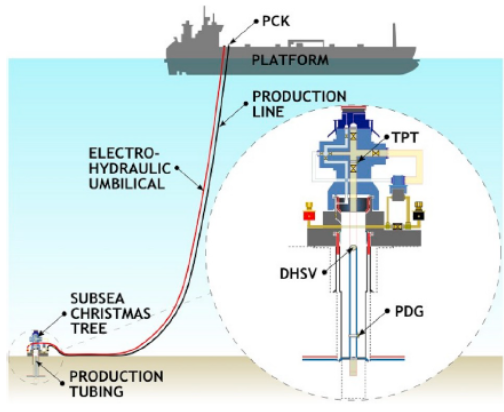
\includegraphics[width=0.6\textwidth]{offshore_well.png}
\caption{\label{fig:offshore_well}Schematic of a typical offshore well}
\end{figure}

In addition to this, Petrobras experts can confirm the issues of each type of undesirable event after considering their distinct time window sizes \parencite{revvargas2019}. For Severe Slugging specifically, the window size was set as 5 hours.


\subsection{Hypothesis}
The data present in 3W Data Set's real instances enables classifier models to detect Severe Slugging with high accuracy, precision and recall.

\subsection{General Goal}
The business objective of our project is to apply machine learning techniques modeled in this project to the 3W data set to accurately detect \emph{Severe Slugging} in an offshore well production line. By identifying the correlations between the variables presented in the records monitored in an offshore oil well operation, this project must present at least one classification model with high accuracy, precision and recall when detecting presence or absence of Severe Slugging. 

\subsection{Success Criteria}
The metrics which are guiding this project are accuracy, precision and recall presented by the models when performing a binary classification to detect the presence or absence of Severe Slugging. 

As stated by \textcite{wegier_ksieniewicz_2020}, the mere use of accuracy as metric for binary classification of imbalanced data does not consider the disparities in the problem classes and therefore misjudges the quality of the model. Adopting recall as a criteria enabled this project to determine the accuracy of the minority class classification - that is, the presence of Severe Slugging - and adopting precision could help the define the  probability of its correct detection.

\subsection{Methodologies and Technologies}

The methodology that guided this project was \emph{CRISP-DM}, which is most widely adopted methodology for data mining, data analytics, and data science projects \parencite{ibm_crisp_dm}. Given this, a number of software libraries and modules were used throughout this process to support some of its distinct stages, that is, Data Understanding, Data Preparation, Modeling, and Evaluation. 

Once the methodology was defined, Petrobras' \emph{3W Tool Kit} was studied and used to extract the data from the instances interesting to the project, that is, from the real instances that effectively presented the Severe Slugging event.

Then, \emph{Pandas} and \emph{NumPy} libraries were selected for data manipulation and analysis. Then, the base machine learning library for the majority of models in this project was \emph{Scikit-learn}, as it offers various pre-processing, classification models and clustering algorithms. Another library imported in this project was \emph{Keras}, which is is an open-source solution that provides an interface for artificial neural networks.

Besides that, \emph{StandardScaler} from the \emph{Scikit-learn} library was selected for scaling and normalisation of the data. Given the high data imbalance presented by the data set, a \emph{RandomUnderSampler} was also from \emph{Imbalanced-learn} library was imported. Regarding feature reduction, the decomposition algorithm \emph{PCA}, also from \emph{Scikit-learn}, was adopted here in this study. 

Also, \emph{Seaborn}, \emph{Matplotlib} and \emph{Plotly} libraries were widely used to analyse data throughout the project and provide data visualisation using at the Evaluation stage. Another tool from \emph{Scikit-learn} selected as a baseline model was \emph{DummyClassifier}. 

Additionally, the following tools from module \emph{model\_selection} in \emph{Scikit-learn} library were chose:

\begin{itemize}
    \item \emph{GridSearchCV}, for hyperparameter tuning
    \item \emph{cross\_val\_score} for cross-validation, 
    \item \emph{train\_test\_split} for train/test splitting,
    \item \emph{KFold} for cross-validation during Evaluation
\end{itemize}

Ultimately, \emph{Scikit-learn} library also provided the following classifiers for this project:
\begin{itemize}
    \item LinearSVC, from \emph{svm} module,
    \item KNeighborsClassifier, from \emph{neighbors} module,
    \item DecisionTreeClassifier, from \emph{tree} module,
    \item RandomForestClassifier, from \emph{ensemble} module
\end{itemize}

Lastly, the modules \emph{make\_pipeline} and \emph{Pipeline} from \emph{Scikit-learn} were used to chain all steps of the workflow together, and the library \emph{Pickle} was selected to persist the resulting models in file.


\subsection{Accomplishment}
After extracting the data using 3W Tool Kit and performing iterations with observance of CRISP-DM, this project managed to find 2 classification models with high accuracy, precision, and recall.

\section{Data Understanding}

Pre-processing a data set through data characterisation involves summarising the features and characteristics present in the data using statistical measures and visualisations techniques such as bar charts and scatter plots. After this stage, it should be possible to identify biases, patterns, trends, and any missing or irrelevant data in the data set that may need to be addressed.

This data set is composed by instances of eight types of undesirable events characterized by eight process variables from three different sources: real instances, simulated instances and hand-drawn instances. All real instances were taken from the plant information system that is used to monitor the industrial processes at an operational unit in Brazilian state of Espírito Santo - namely UO-ES. The simulated instances were all generated using OLGA, a dynamic multi-phase flow simulator that is widely used by oil companies worldwide \parencite{andreolli2016introduccao}. Eventually, the hand-drawn instances were generated by a specific tool developed by Petrobras researchers for this data set to incorporate undesirable events classified as rare.

Ultimately, only the data from the real instances was selected for this project, as simulated instances and hand-drawn instances did not present any record for two features relevant to Severe Slugging, namely Gas Lift Flow Rate (QGL) and Pressure Variable Upstream of the Gas Lift Choke.

According to \textcite{revvargas2019}, the \emph{realistic} aspects of the data present in the 3W data set real instances were kept, since there was no pre-processing. Therefore, NaN values, frozen variables caused by sensor or network communication problems, asymmetrical instances with non-normal distribution of the events and extreme outliers were commonly found. 

These so-called "realistic" aspects of the data were expected by this work, given the complexity of an offshore operation, where a significant amount of variables were collected by sub-sea equipment located miles from the Brazilian coast.

\subsection{Data Collection}
The data used in this study was extracted after following the documentation from 3W took kit \parencite{petrobras3WToolkit}, which is a Python software package with resources to experiment machine learning-based approaches and algorithms for issues related to undesirable events. The specific data used in this study was from the \emph{real instances}, and it was also available at \textcite{extracted3Wcsv} at the time of publication of this study.

\subsection{Data Characterisation}

The selected data set consists of 13,952,911 observations, with 14 columns of data for each observation and the distribution of the \emph{instances}. Every instance contains a variable number of text files representing the data collected in each well and they present the same data structure: the first column, label, indicates the event type for each observation, while second column, well, contains the name of the well the observation was taken from. Hand-drawn and simulated instances have fixed names for in this column, while real instances have names masked with incremental id. The third column, id, is an identifier for the observation and it is incremental for hand-drawn and simulated instances, while each real instance has an id generated from its first timestamp. 

Besides that, the pressure features are measured in Pascal (Pa), the volumetric flow rate features are measured in standard cubic meters per second (SCM/s), and the temperature features are measured in degrees Celsius (°C). In order to maintain the realistic aspects of the data, the data set was built without pre-processing, including the presence of NaN values, frozen variables due to sensor or communication issues, instances with varying sizes, and outliers \parencite{revvargas2019}, which demanded further processing as described in the next sections.

\begin{itemize}
\item label: instance label (event type) - target variable;
\item well: well name. Hand-drawn and simulated instances have fixed names (respectively, drawn and simulated. Real instances have names masked with incremental id;
\item id: instance identifier. Hand-drawn and simulated instances have incremental id. Each real instance has an id generated from its first timestamp;
\item class: Although it can be used to identify periods of normal operation, fault transients, and faulty steady states, which can help with diagnosis and maintenance, it is a category which results from label, which is our target here
\end{itemize}

A concise summary of this data set generated by \emph{pandas.DataFrame.info} method can be seen on Table ~\ref{tab:widgets}.

\begin{table}
\centering
\begin{tabular}{l|r|r}

Column & pandas.Dtype & Description\\\hline
timestamp & datetime64[ns] & timestamp \\
label & int64 & label \\        
well & object & well \\       
id & int64 & id \\        
P-PDG & float64 & pressure variable at the PDG, in Pa \\      
P-TPT & float64 & pressure variable at the TPT, in Pa \\     
T-TPT & float64 & temperature variable at the TPT, in °C \\      
P-MON-CKP & float64 & pressure variable upstream of CKP, in Pa \\      
T-JUS-CKP & float64 & temperature variable downstream of CKP, in °C \\      
P-JUS-CKGL & float64 & pressure variable upstream of CKGL, in °C \\       
T-JUS-CKGL & float64 & temperature variable upstream of CKGL,  in °C\\     
QGL & float64 & gas life flow rate, SCM/s\\      
class & float64 & operation state: normal, fault, faulty steady \\   
source & object & type of instance: real, simulated or hand-drawn \\     

\end{tabular}
\caption{\label{tab:widgets}Summary of the data set compiled from real instances}
\end{table}




\begin{table}[h]
\centering
\begin{tabular}{lrrr|r}

INSTANCE LABEL & REAL & SIMULATED & HAND-DRAWN & TOTAL \\ \hline
0 - Normal Operation & 597 & 0 & 0 & 597 \\
1 - Abrupt Increase of BSW & 5 & 114 & 10 & 129 \\
2 - Spurious Closure of DHSV & 22 & 16 & 0 & 38 \\
3 - Severe Slugging & 32 & 74 & 0 & 106 \\
4 - Flow Instability & 344 & 0 & 0 & 344 \\
5 - Rapid Productivity Loss & 12 & 439 & 0 & 451 \\
6 - Quick Restriction in PCK & 6 & 215 & 0 & 221 \\
7 - Scaling in PCK & 4 & 0 & 10 & 14 \\
8 - Hydrate in Production Line & 0 & 81 & 0 & 81 \\
\hline
\textbf{TOTAL} & 1022 & 939 & 20 & 1981 \
\end{tabular}
\caption{Data distribution in the different sources and instance labels.}
\label{tab:data_distribution}
\end{table}


The values for all undesirable events found in the data set in column \emph{label} are:

\begin{itemize}
\item 0 - Normal Operation = Normal
\item 1 - Abrupt Increase of BSW = AbrIncrBSW
\item 2 - Spurious Closure of DHSV = SpurClosDHSW
\item 3 - Severe Slugging = SevSlug
\item 4 - Flow Instability = FlowInst
\item 5 - Rapid Productivity Loss = RProdLoss
\item 6 - Quick Restriction in PCK = QuiRestrPCK
\item 7 - Scaling in PCK = ScalingPCK
\item 8 - Hydrate in Production Line = HydrProdLine
\end{itemize}

\subsection{Exploratory Data Analysis}

A bar chart was generated displaying the percentage of present values in each column of the data frame - see Figure \ref{fig:missingvalues}. The data set contained missing values in several columns, thus some columns and row were deleted in order to obtain accurate and reliable results.

Three boxplots were plotted to show how the data was distributed before any data cleaning - see Figure \ref{fig:distr_boxplots_before_cleaning}. They were divided according the feature measurement unit: the pressure features were measured in Pascal (Pa), the temperature features are measured in degrees Celsius (°C) and one feature about volumetric flow rate which was measured in standard cubic meters per second (SCM/s).

\begin{figure}
\centering
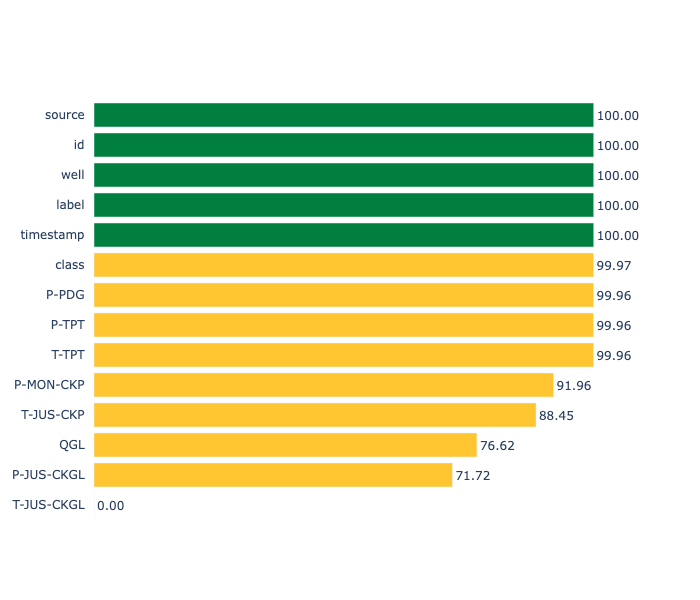
\includegraphics[width=1\textwidth]{missingvalues.png}
\caption{\label{fig:missingvalues}Proportion of available data per column, in \%.}
\end{figure}


\begin{figure}
\centering
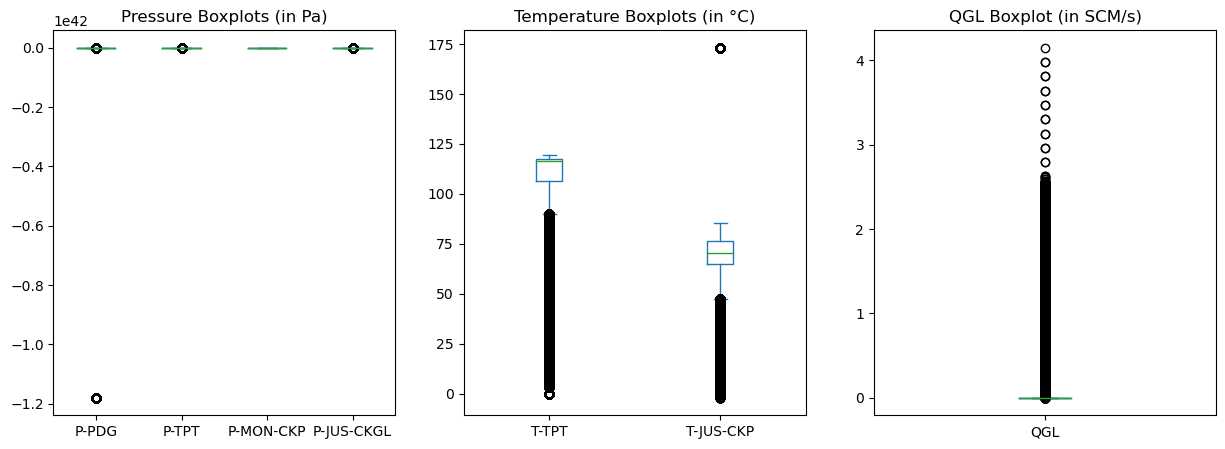
\includegraphics[width=1\textwidth]{distr_boxplots_before_cleaning.png}
\caption{\label{fig:distr_boxplots_before_cleaning}Box plots showing the distribution of pressure, temperature, and QGL (SCM/s) data for a set of oil wells.}
\end{figure}

The distribution of the undesirable events in the real instances of 3W Data Set can be visualised on Figure \ref{fig:undesirable_event_distr}

\begin{figure}
\centering
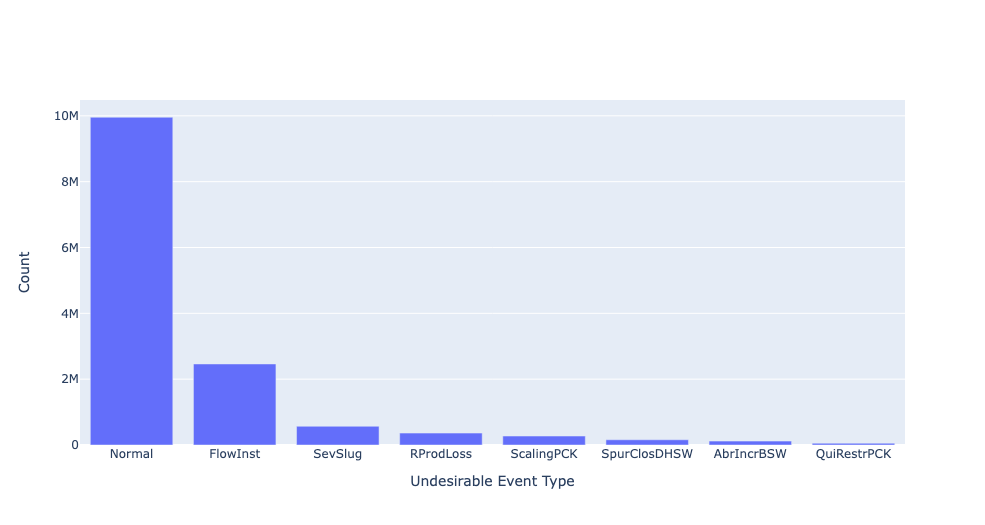
\includegraphics[width=1\textwidth]{undesirable_event_distr.png}
\caption{\label{fig:undesirable_event_distr}Distribution of the undesirable events in the real instances.}
\end{figure}


\section{Data Preparation}

Data preparation included Data Cleaning, Feature Engineering, Train/Test Splitting and Handling Imbalanced Data, Data Scaling, and an analysis of the chosen approach regarding dimensionality reduction for some models.

\subsection{Data Cleaning}

The missing data from the following columns were removed: class, P-PDG, P-TPT, T-JUS-CKP, P-MON-CKP,T-TPT, P-MON-CKP, QGL and P-JUS-CKGL. After this, the columns class, T-JUS-CKGL (an empty column), id, source were dropped. Column class is a column which brings more details about label. Consider that columns timestamp, label were kept at this stage. Finally all duplicates were removed. 

\begin{lstlisting}[language=Python]
# dropping rows with missing or null class column
df_clean = df.dropna(subset=[
    'class','P-PDG','P-TPT','T-JUS-CKP','P-MON-CKP','T-TPT',
    'P-MON-CKP','QGL','P-JUS-CKGL'
])

# removing redundant columns
df_clean = df_clean.drop(['class','T-JUS-CKGL','id','source'], axis=1)

# checking duplicated rows after removing ids
df_clean = df_clean.drop_duplicates()

df_clean.info()
\end{lstlisting}

\begin{verbatim}
<class 'pandas.core.frame.DataFrame'>
Int64Index: 10003580 entries, 0 to 13952910
Data columns (total 10 columns):
 #   Column      Dtype         
---  ------      -----         
 0   timestamp   datetime64[ns]
 1   label       int64         
 2   well        object        
 3   P-PDG       float64       
 4   P-TPT       float64       
 5   T-TPT       float64       
 6   P-MON-CKP   float64       
 7   T-JUS-CKP   float64       
 8   P-JUS-CKGL  float64       
 9   QGL         float64       
dtypes: datetime64[ns](1), float64(7), int64(1), object(1)
memory usage: 839.5+ MB
\end{verbatim}

Also, as it can be seen on Figure \ref{fig:distr_boxplots_before_cleaning}, features P-PDG and P-TPT had the presence of extreme outliers. These outliers were also removed with the following code:

\begin{lstlisting}[language=Python]
# removing extreme outliers from P-PDG 
Q1 = df_clean['P-PDG'].quantile(0.25)
Q3 = df_clean['P-PDG'].quantile(0.75)
IQR = Q3 - Q1
lower_bound = Q1 - (3 * IQR)
df_no_outliers = df_clean[(df_clean['P-PDG'] >= lower_bound)]

# removing extreme outliers from P-TPT
Q1 = df_no_outliers['P-TPT'].quantile(0.25)
Q3 = df_no_outliers['P-TPT'].quantile(0.75)
IQR = Q3 - Q1
upper_bound = Q3 + (3 * IQR)
df_no_outliers = df_no_outliers[(df_no_outliers['P-TPT'] <= upper_bound)]

df_no_outliers.shape
\end{lstlisting}
\begin{verbatim}
(9780901, 10)
\end{verbatim}

These rows with presence of extreme outliers represented 2.26\% of the resulting rows so far. As a result the distribution of values in P-PDG and P-TPT were modified, as Figure \ref{fig:distr_boxplots_after_cleaning} shows.

\begin{figure}
\centering
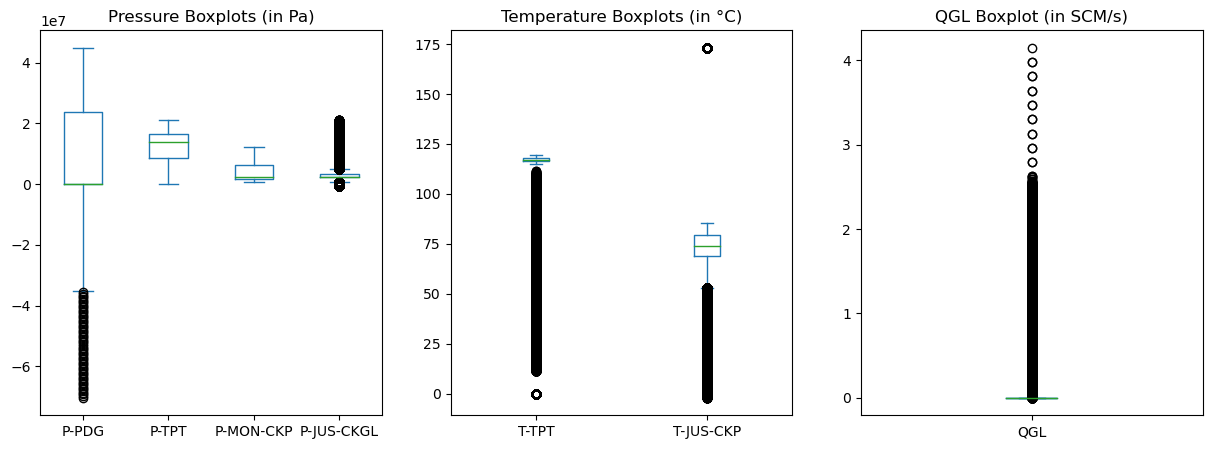
\includegraphics[width=1\textwidth]{distr_boxplots_after_cleaning.png}
\caption{\label{fig:distr_boxplots_after_cleaning}Box plots showing the distribution of pressure, temperature, and QGL (SCM/s) data without extreme outliers.}
\end{figure}


\subsection{Feature Engineering}

Given the label feature contains 8 possible numeric labels for each undesirable event and 1 label value 0 for normal observations, 8 new boolean columns were created for each one undesirable event, including for Severe Slugging, which is this project's target.

\begin{lstlisting}[language=Python]
dt_feat = df_no_outliers

# Changing 'label' column to object dtype
dt_feat['label'] = dt_feat['label'].astype('object') 

# Creating uint8 columns for each label
label_dummies = pd.get_dummies(dt_feat['label'], prefix='label')
dt_feat = pd.concat([dt_feat, label_dummies], axis=1)

# Renaming uint8 columns
column_names = {
    'label_0': 'Normal',
    'label_1': 'AbrIncrBSW',
    'label_2': 'SpurClosDHSW',
    'label_3': 'SevSlug', # target
    'label_4': 'FlowInst',
    'label_5': 'RProdLoss',
    'label_6': 'QuiRestrPCK',
    'label_7': 'ScalingPCK',
    'label_8': 'HydrProdLine'
}
dt_feat = dt_feat.rename(columns=column_names)

# Dropping the original 'label' column and Normal column, 
# since all other events must be 0
dt_feat = dt_feat.drop(['label','Normal'], axis=1)
dt_feat.info()
\end{lstlisting}
\begin{verbatim}
<class 'pandas.core.frame.DataFrame'>
Int64Index: 9780901 entries, 0 to 13952910
Data columns (total 16 columns):
 #   Column        Dtype         
---  ------        -----         
 0   timestamp     datetime64[ns]
 1   well          object        
 2   P-PDG         float64       
 3   P-TPT         float64       
 4   T-TPT         float64       
 5   P-MON-CKP     float64       
 6   T-JUS-CKP     float64       
 7   P-JUS-CKGL    float64       
 8   QGL           float64       
 9   AbrIncrBSW    uint8         
 10  SpurClosDHSW  uint8         
 11  SevSlug       uint8         
 12  FlowInst      uint8         
 13  RProdLoss     uint8         
 14  QuiRestrPCK   uint8         
 15  ScalingPCK    uint8         
dtypes: datetime64[ns](1), float64(7), object(1), uint8(7)
memory usage: 811.5+ MB
\end{verbatim}

Then all undesirable events columns were deleted but the column which denotes the observations presents Severe Slugging. The column \emph{HydrProdLine} concerned to Hydrate in Production line, however this event was not found in the data set resulting from real instances.

\begin{lstlisting}[language=Python]
dt_feat_target = dt_feat.drop([
#     , 'SevSlug', 'HydrProdLine',
    'AbrIncrBSW','SpurClosDHSW','FlowInst','RProdLoss','QuiRestrPCK','ScalingPCK'
], axis=1)

dt_feat_target.info()
\end{lstlisting}
\begin{verbatim}
<class 'pandas.core.frame.DataFrame'>
Int64Index: 9780901 entries, 0 to 13952910
Data columns (total 10 columns):
 #   Column      Dtype         
---  ------      -----         
 0   timestamp   datetime64[ns]
 1   well        object        
 2   P-PDG       float64       
 3   P-TPT       float64       
 4   T-TPT       float64       
 5   P-MON-CKP   float64       
 6   T-JUS-CKP   float64       
 7   P-JUS-CKGL  float64       
 8   QGL         float64       
 9   SevSlug     uint8         
dtypes: datetime64[ns](1), float64(7), object(1), uint8(1)
memory usage: 755.6+ MB
\end{verbatim}

\subsection{Train/Test Splitting}

The following code defined how the data set was split in Train and Test data sets. Additionally, the columns \emph{timestamp} and \emph{well} were removed and at the end the  distribution of the records according the presence or absence of Severe Slugging was computed.

\begin{lstlisting}[language=Python]
# defining features (X) and label (y)
target = 'SevSlug'

X = dt_feat_target.drop([target,'timestamp','well'], axis=1)
y = dt_feat_target[target]

# splitting data into train and test sets
X_train_u, X_test, y_train_u, y_test = train_test_split(X, y, test_size=0.3, random_state=42)

class_names = {0:'Non Sev Slug', 1:'SEV SLUGGING'}
print(y_train_u.value_counts(normalize=True).rename(index=class_names))
\end{lstlisting}
\begin{verbatim}
Non Sev Slug    0.94194
SEV SLUGGING    0.05806
Name: SevSlug, dtype: float64
\end{verbatim}

After the splitting process, the training data set had 6,846,630 rows and the test data set had 2,934,271 rows.

\subsection{Handling Imbalanced Data}

A \emph{RandomUnderSampler} was chosen to balance training data. As a result 50\% of observations presented Severe Slugging while the other 50\% were normal or presented other undesirable event. Test data set was not balanced since this work aim to best represent your deployment scenarios in real life.

\begin{lstlisting}[language=Python]
# balancing data 
balancing = RandomUnderSampler(random_state=42)

X_train, y_train = balancing.fit_resample(X_train_u, y_train_u)

class_names = {0:'Non Sev Slug', 1:'SEV SLUGGING'}
print(y_train.value_counts(normalize=True).rename(index=class_names))
print([X_train.shape, y_train.shape])
\end{lstlisting}
\begin{verbatim}
Non Sev Slug    0.5
SEV SLUGGING    0.5
Name: SevSlug, dtype: float64
[(795026, 7), (795026,)]
\end{verbatim}

Handling data imbalance is also important because it affects correlations - see as Figure \ref{fig:correlations} shows.

\begin{figure}
\centering
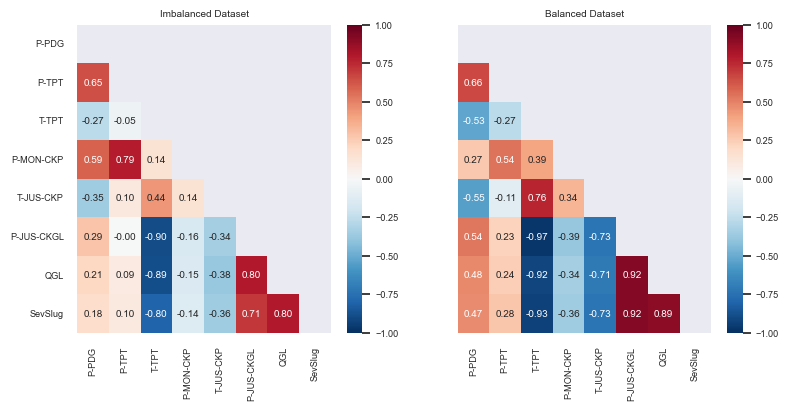
\includegraphics[width=1\textwidth]{correlations.png}
\caption{\label{fig:correlations}Correlations between variables before and after data balancing}
\end{figure}

\subsection{Data Scaling}

Although there are features presenting non-normal distributions, \emph{StandardScaler} was chosen as data scaler. It was chose because there are some features with strong correlation with Severe Slugging and lognormal distributions such as \emph{QGL} and \emph{P-JUS-CKGL} and as it is a method sensitive to the presence of outliers. The results of this transformation can be seen on Figure \ref{fig:std_scaler}.

\begin{figure}
\centering
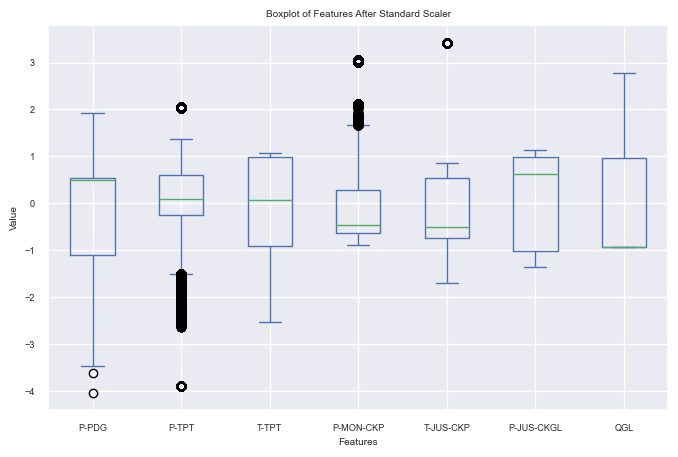
\includegraphics[width=1\textwidth]{std_scaler.png}
\caption{\label{fig:std_scaler}Box plot showing the distribution of the features in the training set after applying the StandardScaler transformation}
\end{figure}


\subsection{Dimensionality Reduction}

The unsupervised learning technique Principal Component Analysis (PCA) was chosen not only to prepare the data for some of the models studied here, but also to evidence any possible linear separability in this model. In Figure \ref{fig:pca} the results of this dimensionality reduction can be seen in two ways, with 2 and 3 components, although this process was unnecessary for the most successful models, that is, the non-linear classifiers.

\begin{figure}
\centering
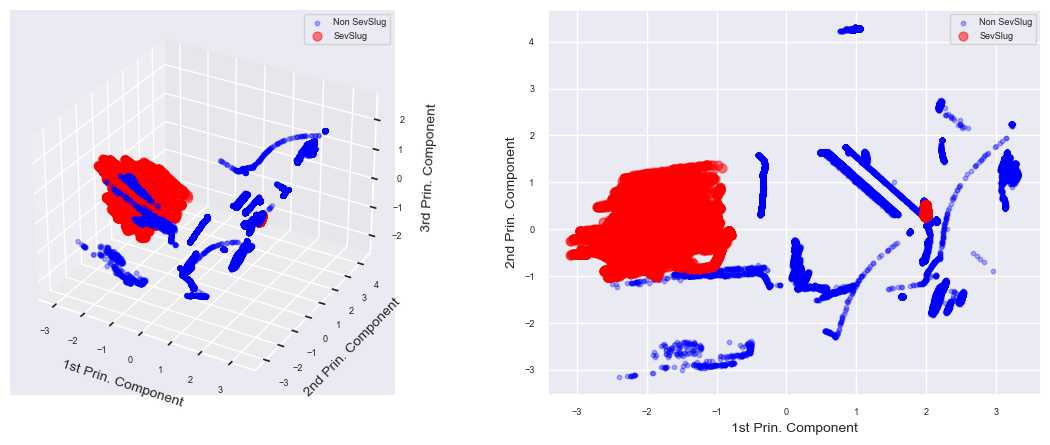
\includegraphics[width=1\textwidth]{pca.png}
\caption{\label{fig:pca}Visualisation of PCA applied to the data set showing a scatter plot for two (2D) and three (3D) principal components.}
\end{figure}

\section{Modeling}

As stated by \textcite{venkatasubramanian_rengaswamy_yin_kavuri_2003}, the abnormal event management (AEM) includes detection of an event, analysing its root cause and taking the suitable control decisions and measures to bring the situation into a normal, safe and operational condition. Additionally, an automated AEM should handle diagnosis of an event as a classification task.

Given this, five models were chosen for this project: LinearSVC, k-Nearest Neighbors Classifier, Artificial Neural Network, Decision Tree Classifier and Random Forest Classifier. 

\subsection{Baseline: DummyClassifier}
Before proceeding with other models, a DummyClassifier was adopted to find a baseline for validation accuracy using the test data set. Given the distribution of the target variable in test data set, the baseline for any model was set in 94.17\%.

\begin{lstlisting}[language=Python]
dummy_pipeline = make_pipeline(StandardScaler(), DummyClassifier())
dummy_pipeline.fit(X_train, y_train)

# confirming score for Dummy classifier results from a balanced dataset
score = dummy_pipeline.score(X_train, y_train)

# predicting
y_predicted = dummy_pipeline.predict(X_test)
baseline = metrics.accuracy_score(y_test, y_predicted)

print("Score: ", score)
print("Accuracy: ",baseline)
\end{lstlisting}
\begin{verbatim}
Score:  0.5
Accuracy:  0.9417780429960286
\end{verbatim}

\subsection{LinearSVC}
Although the data is not linearly separable and it is not possible to find a condition of 100\% correctly classified by a hyperplane, a linear support vector classifier (LinearSVC) was implemented as part of this benchmark. The code below retrieved a previously trained LinearSVC model which was persisted as a Pickle file, then it predicted the class labels for the features in \emph{X\_test}, and finally generated the respective Classification Report in comparison with the labels in \emph{y\_test}.

\begin{lstlisting}[language=Python]
with open(os.path.join('pickle', 'linear_svc_pipeline.pkl'), 'rb') as f:
linear_svc_pipeline = pickle.load(f)
    
y_predicted_lin_clf = linear_svc_pipeline.predict(X_test)    

cr_linearsvc = metrics.classification_report(y_test, y_predicted_lin_clf, digits=4)
\end{lstlisting}

\subsubsection{Hyperparameter optimisation}
For finding the best parameters for this model, the hyperparameters to tune PCA and the model were specified. Then a pipeline was created with 3 steps:
\begin{enumerate}
\item \emph{scaler} which uses StandardScaler method to scale the data
\item \emph{dimred} which applies PCA dimensionality reduction
\item \emph{linearsvc} which applies the LinearSVC model.
\end{enumerate}

At this point, a grid search was performed using the above-mentioned pipeline and the hyperparameter grid to find the combination with the best f1 metric with the default cross-validation, that is, a 5-fold cross-validation. Also, the parameter \emph{class\_weight} was listing possible 2 values (\emph{balanced} and \emph{None}) during hyperparametrisation tuning, since the "balanced" mode considers \emph{y} values to adjust the weights inversely proportional to the class frequencies in the input data, which is effectively balanced at this point for this model.

\begin{lstlisting}[language=Python]
from sklearn.svm import LinearSVC

param_grid = {
    'dimred__n_components': [3, 4], 
    'linearsvc__C': [1e-2, 1e-1, 1, 10, 100],
    'linearsvc__penalty':['l1', 'l2'],
    'linearsvc__dual': [False, True],
    'linearsvc__class_weight': ['balanced', None]
}

linear_svc_pipeline = Pipeline([
    ('scaler', scaler_pipeline), 
    ('dimred', PCA()), 
    ('linearsvc', LinearSVC())
])

grid_search_lsvc = GridSearchCV(
    linear_svc_pipeline,
    param_grid=param_grid,
    n_jobs=-1,
    scoring='f1',
    verbose=1
)

grid_search_lsvc.fit(X_train, y_train)
\end{lstlisting}

After this, the pipeline was defined with the best parameters found:
\begin{enumerate}
    \item StandardScaler()
    \item PCA(n\_components=3)
    \item LinearSVC(C=0.01, class\_weight='balanced', dual=False, penalty='l1')
\end{enumerate}

\subsubsection{Model training}
Then the model was trained using a similar pipeline, but this time with the optimal combination of parameters.

\begin{lstlisting}[language=Python]
linear_svc_pipeline = Pipeline([
    ('scaler', scaler_pipeline), 
    ('dimred', PCA(
        n_components=grid_search_lsvc.best_params_['dimred__n_components']
    )),
    ('linearsvc', LinearSVC(
        dual=grid_search_lsvc.best_params_['linearsvc__dual'],
        C=grid_search_lsvc.best_params_['linearsvc__C'],
        penalty=grid_search_lsvc.best_params_['linearsvc__penalty'],
        class_weight=grid_search_lsvc.best_params_['linearsvc__class_weight']
    ))
])

linear_svc_pipeline.fit(X_train, y_train)
\end{lstlisting}

\subsection{k-Nearest Neighbors Classifier}
A k-Nearest Neighbors Classifier (KNeighborsClassifier) was implemented as part of this benchmark. The code below retrieved a previously trained KNeighborsClassifier model which was persisted as a Pickle file, then it predicted the class labels for the features in \emph{X\_test}, and finally generated the respective Classification Report in comparison with the labels in \emph{y\_test}.

\begin{lstlisting}[language=Python]
with open(os.path.join('pickle', 'knn_pipeline.pkl'), 'rb') as f:    
    knn_pipeline = pickle.load(f)
    
y_predicted_knn = knn_pipeline.predict(X_test)

cr_knn = metrics.classification_report(y_test, y_predicted_knn, digits=5)    
\end{lstlisting}

\subsubsection{Hyperparameter optimisation}
For finding the best parameters for this model, the hyperparameters to tune PCA and the model were specified. Then a pipeline was created with 3 steps:
\begin{enumerate}
\item \emph{scaler} which uses StandardScaler method to scale the data
\item \emph{dimred} which applies PCA dimensionality reduction
\item \emph{kneighborsclassifier} which applies the KNeighborsClassifier model.
\end{enumerate}

Finally, a grid search was performed using the above-mentioned pipeline and the hyperparameter grid to find the combination with the best accuracy metric with the default cross-validation, that is, a 5-fold cross-validation.
\begin{lstlisting}[language=Python]
from sklearn.neighbors import KNeighborsClassifier

knn_pipeline = Pipeline([
    ('scaler', scaler_pipeline), 
    ('dimred', PCA()), 
    ('kneighborsclassifier', KNeighborsClassifier())
])

param_grid = {
    'dimred__n_components': [3, 4], 
    'kneighborsclassifier__n_neighbors': range(3, 102, 3),
}

grid_search_knn = GridSearchCV(
    knn_pipeline,
    param_grid=param_grid,
    n_jobs=-1,
    scoring='f1',
    verbose=1
)

grid_search_knn.fit(X_train, y_train)
\end{lstlisting}

Then, the pipeline was redefined with the best parameters found considering the proposed scenario:
\begin{enumerate}
    \item StandardScaler()
    \item PCA(n\_components=4)
    \item KNeighborsClassifier(n\_neighbors=3)
\end{enumerate}

\subsubsection{Model training}
Then the model was trained using a similar pipeline, but this time with the optimal combination of parameters.

\begin{lstlisting}[language=Python]
knn_pipeline = Pipeline([
    ('scaler', scaler_pipeline), 
    ('dimred', PCA(
        n_components=grid_search_knn.best_params_['dimred__n_components']
    )),
    ('kneighborsclassifier', KNeighborsClassifier(
        n_neighbors=grid_search_knn.best_params_['kneighborsclassifier__n_neighbors']
    ))
])


knn_pipeline.fit(X_train, y_train)
\end{lstlisting}

Although the risk of over-fitting was relatively unlikely given the minimal configuration used in this model, a comparison between the f1 score in training and test data sets according the \emph{n\_neighbors} was implemented below. This chart is visible on Figure \ref{fig:knn_overfitting}.

\begin{lstlisting}[language=Python]
# initialising arrays for storing train and test accuracy
neighbors = np.arange(3, 103, 10)     
knn_train_f1_score = np.zeros(len(neighbors))    
knn_test_f1_score = np.zeros(len(neighbors))    

# looping over different values of k
for i, k in enumerate(neighbors):     
    knn_pipeline_ = Pipeline([
        ('scaler', scaler_pipeline), 
        ('dimred', PCA(n_components=4)), 
        ('kneighborsclassifier', KNeighborsClassifier(n_neighbors=k))
    ])
    
    knn_pipeline_.fit(X_train, y_train)                             
    y_pred_train = knn_pipeline_.predict(X_train)
    y_pred_test = knn_pipeline_.predict(X_test)
    
    knn_train_f1_score[i] = f1_score(y_train, y_pred_train)    
    knn_test_f1_score[i] = f1_score(y_test, y_pred_test)   
\end{lstlisting}

\begin{lstlisting}[language=Python]
# creating figure, adding title
plt.figure(figsize = (10, 6))

# plotting the test accuracy and traning accuracy x number of neighbours
plt.plot(neighbors, knn_test_f1_score, label = 'Testing F1')
plt.plot(neighbors, knn_train_f1_score, label = 'Training F1')

# adding legend, axes labels, setting font size and axes ticks
plt.legend(prop={'size': 10})
plt.xlabel('Number of neighbors', fontsize = 10)
plt.ylabel('F1 Score', fontsize = 10)
plt.xticks(fontsize = 10)
plt.yticks(fontsize = 10)

plt.show()
\end{lstlisting}

\begin{figure}
\centering
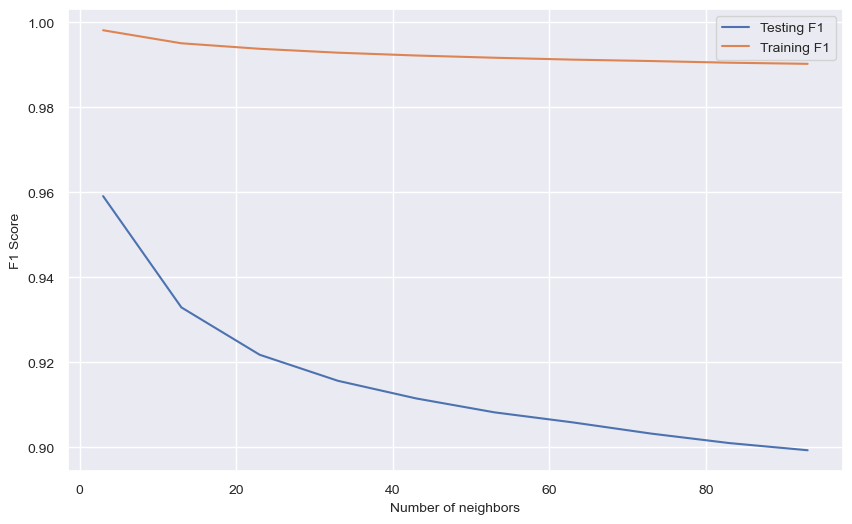
\includegraphics[width=0.8\textwidth]{knn_overfitting.png}
\caption{\label{fig:knn_overfitting}Comparison between training and test f1 score according the number of neighbours in k-Neighbours Classifier}
\end{figure}

\subsection{Artificial Neural Network}

In this subsection, \emph{Keras} and \emph{Tensorflow} libraries were used to define a baseline model using Artificial Neural Network (ANN). Similar to previous models, the code below could retrieve a previously trained ANN model which was persisted as a Pickle file, then it predicted the class labels for the features in \emph{X\_test} after normalisation and adjusting the data type using \emph{Numpy} function. After this, the corresponding Classification Report in comparison with the labels in \emph{y\_test} was generated. 

\begin{lstlisting}[language=Python]
import tensorflow as tf
from tensorflow import keras
from keras import backend as K

BATCH_SIZE = 2048

with open(os.path.join('pickle', 'ann_model.pkl'), 'rb') as f: 
    ann_model_ = pickle.load(f)
    
scaler = StandardScaler()    

X_test_scaled = scaler.fit_transform(X_test)

y_predicted_ann = ann_model_.predict(np.array(X_test_scaled), batch_size=BATCH_SIZE)
y_predicted_ann = y_predicted_ann.flatten()
y_predicted_ann = np.where(y_predicted_ann.round(2) > 0.5, 1, 0)

cr_ann = metrics.classification_report(y_test, y_predicted_ann, digits=5)    
\end{lstlisting}
\begin{verbatim}
1433/1433 [==============================] - 1s 777us/step
\end{verbatim}

Also the parameter \emph{batch\_size} was set as 2048, a relatively high value for this parameter, but capable to increase the chance of having some positive samples in each batch.

\subsubsection{Data Preparation for Keras}

For this model, a distinct approach to prepare the data set was adopted. Firstly, the original imbalanced clean data set was copied and split with the same parameter \emph{random\_state=42} used to generate the training data set used to fit and test the other models in this work. Secondly, the resulting train data set from this process was split again into train set and validation set.

Then, the validation set was only used during the model fitting to evaluate the loss, precision, recall and accuracy - however the model was not fit with this data. As a consequence, the test set was completely isolated during the training stage and was only used to evaluate how well the model generalizes to new data. 

This approach is highly recommended to avoid over-fitting, which is a constant concern due to a possible lack of training data in imbalanced data sets \parencite{tensorflow2015-whitepaper} like the one used in this project, where the number of examples not presenting Severe Slugging class greatly outnumbered the examples presenting it.

Given this, the processes adopted for the data set in this section for data cleaning and scaling were the same processes adopted for the other models in this work, however the data is not balanced at this points. These adjustments were necessary to fulfill the requirements of a similar model described in TensorFlow Tutorial provided by \textcite{tensorflow2015-whitepaper}. The code that had performed these tasks can be see below. 

\begin{lstlisting}[language=Python]
ann_df = df_feat.copy() # copying the imbalanced but clean data set

non_sev_slug, sev_slug = np.bincount(ann_df['SevSlug'])

total = non_sev_slug + sev_slug
print('Examples:\n    Total: {}\n    SevSlug: {} ({:.2f}% of total)\n'.format(
    total, sev_slug, 100 * sev_slug / total))
\end{lstlisting}
\begin{verbatim}
Examples:
    Total: 9780901
    SevSlug: 568352 (5.81% of total)
\end{verbatim}

\begin{lstlisting}[language=Python]
# Dropping redundant columns for this project
ann_df.pop('timestamp')
ann_df.pop('well')
ann_df.columns
\end{lstlisting}
\begin{verbatim}
Index(['P-PDG', 'P-TPT', 'T-TPT', 'P-MON-CKP', 'T-JUS-CKP', 'P-JUS-CKGL',
       'QGL', 'SevSlug'],
      dtype='object')
\end{verbatim}

\begin{lstlisting}[language=Python]
# Splitting data
ann_train_df, ann_test_df = train_test_split(ann_df, test_size=0.3, random_state=42)
ann_train_df, ann_val_df = train_test_split(ann_train_df, test_size=0.3)

# Form np arrays of labels and features
train_labels = np.array(ann_train_df.pop('SevSlug'))
bool_train_labels = train_labels != 0
val_labels = np.array(ann_val_df.pop('SevSlug'))
test_labels = np.array(ann_test_df.pop('SevSlug'))

train_features = np.array(ann_train_df)
val_features = np.array(ann_val_df)
test_features = np.array(ann_test_df)
\end{lstlisting}

\begin{lstlisting}[language=Python]
# Normalising data with a previously instantiated StandardScaler
train_features = scaler.fit_transform(train_features)
val_features = scaler.transform(val_features)
test_features = scaler.transform(test_features)

print('ANN Training labels shape:', train_labels.shape)
print('ANN Validation labels shape:', val_labels.shape)
print('Test labels shape:', test_labels.shape)

print('ANN Training features shape:', train_features.shape)
print('ANN Validation features shape:', val_features.shape)
print('Test features shape:', test_features.shape)
\end{lstlisting}
\begin{verbatim}
ANN Training labels shape: (4792641,)
ANN Validation labels shape: (2053989,)
Test labels shape: (2934271,)
ANN Training features shape: (4792641, 7)
ANN Validation features shape: (2053989, 7)
Test features shape: (2934271, 7)
\end{verbatim}

\subsubsection{Model definition}
Instead of using GridSearchCV to tune hyper-parameters like in other models in this project, an initial model was defined and then after analysing its results the initial bias was fixed. Then the model was trained again and had its resulting metrics evaluated considering the validation data set. In the following code the implementation of this initial model is described after listing some metrics available in Keras library that were used to evaluate the model.  

The architecture of this model is visible on Figure \ref{fig:nn_plot} and it has one input layer representing all 7 features from the data set, one densely connected hidden layer with 16 units, a dropout layer to mitigate over-fitting and an one-unit output layer that returns the probability of Severe Slugging.

\begin{lstlisting}[language=Python]
ANN_METRICS = [
    keras.metrics.TruePositives(name='tp'),
    keras.metrics.FalsePositives(name='fp'),
    keras.metrics.TrueNegatives(name='tn'),
    keras.metrics.FalseNegatives(name='fn'), 
    keras.metrics.BinaryAccuracy(name='accuracy'),
    keras.metrics.Precision(name='precision'),
    keras.metrics.Recall(name='recall'),
    keras.metrics.AUC(name='auc'),
    keras.metrics.AUC(name='prc', curve='PR'), # precision-recall curve
]

def make_model(metrics=ANN_METRICS, output_bias=None):
    if output_bias is not None:
        output_bias = tf.keras.initializers.Constant(output_bias)
    model = keras.Sequential([
        keras.layers.Dense(16, activation='relu',input_shape=(train_features.shape[-1],)),
        keras.layers.Dropout(0.5),
        keras.layers.Dense(1, activation='sigmoid',bias_initializer=output_bias),
    ])

    model.compile(
        optimizer=keras.optimizers.Adam(learning_rate=1e-3),
        loss=keras.losses.BinaryCrossentropy(),
        metrics=metrics)

    return model
\end{lstlisting}

The number of epochs used as a reference for this model in this work was 100, however it was not reached, because a resource called \emph{EarlyStopping} was implemented to interrupt the training if a monitored metric has stopped improving. In this resource, the parameter \emph{patience} can be set to make the training more tolerant to possible oscillations in the monitored metric throughout the epochs and the monitored metric here is the \emph{validation precision-recall curve}, which evidences the trade-off between precision and recall for different threshold.

\begin{lstlisting}[language=Python]
EPOCHS = 100

early_stopping = tf.keras.callbacks.EarlyStopping(
    monitor='val_prc', 
    verbose=1,
    patience=10,
    mode='max',
    restore_best_weights=True)

ann_model = make_model()
ann_model.summary()
\end{lstlisting}
\begin{verbatim}
Model: "sequential_5"
_________________________________________________________________
 Layer (type)                Output Shape              Param #   
=================================================================
 dense_10 (Dense)            (None, 16)                128       
                                                                 
 dropout_5 (Dropout)         (None, 16)                0         
                                                                 
 dense_11 (Dense)            (None, 1)                 17        
                                                                 
=================================================================
Total params: 145 (580.00 Byte)
Trainable params: 145 (580.00 Byte)
Non-trainable params: 0 (0.00 Byte)
\end{verbatim}



\begin{figure}
\centering
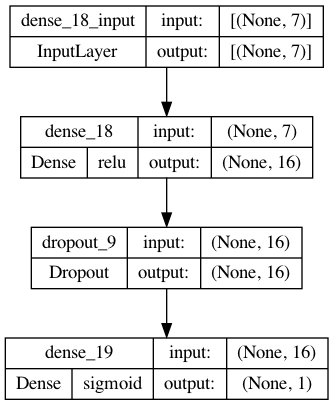
\includegraphics[width=0.35\textwidth]{nn_plot.png}
\caption{\label{fig:nn_plot}The architecture of a neural network model built using Keras}
\end{figure}

Finally, the newly-created model could be briefly tested:

\begin{lstlisting}[language=Python]
ann_model.predict(train_features[:10])
\end{lstlisting}
\begin{verbatim}
1/1 [==============================] - 0s 99ms/step
array([[0.21003543],
       [0.61643285],
       [0.6023897 ],
       [0.62401986],
       [0.62409544],
       [0.21703976],
       [0.2112424 ],
       [0.62370116],
       [0.6251195 ],
       [0.6153809 ]], dtype=float32)
\end{verbatim}

\subsubsection{Handling The Model Bias}
Since the data set is imbalanced, there was an inherent bias in the first results. Given this default bias, the loss can be computed as in the following code:

\begin{lstlisting}[language=Python]
results = ann_model.evaluate(train_features, train_labels, batch_size=BATCH_SIZE, verbose=0)
print("Loss: {:0.4f}".format(results[0]))
\end{lstlisting}
\begin{verbatim}
Loss: 0.9903
\end{verbatim}

The correct bias can be computed as in the following code:
\begin{lstlisting}[language=Python]
initial_bias = np.log([sev_slug / non_sev_slug]) 
initial_bias
\end{lstlisting}
\begin{verbatim}
array([-2.78558091])
\end{verbatim}

Once the initial bias was computed, the model presented more reasonable initial guesses.
\begin{lstlisting}[language=Python]
ann_model = make_model(output_bias=initial_bias)
ann_model.predict(train_features[:10])
\end{lstlisting}
\begin{verbatim}
1/1 [==============================] - 0s 55ms/step
array([[0.03573601],
       [0.03519705],
       [0.03306021],
       [0.04497113],
       [0.045381  ],
       [0.03489733],
       [0.03468524],
       [0.04532901],
       [0.04532651],
       [0.03519929]], dtype=float32)
\end{verbatim}

As a result, the loss was significantly reduced in comparison to the loss found with the naive initialisation, that is, it was reduced from 0.9903 to 0.1167 - see the code below. Additionally, the model did not have to spend the first epochs registering that Severe Slugging only occurred in the minority of the records.

\begin{lstlisting}[language=Python]
results = ann_model.evaluate(train_features, train_labels, batch_size=BATCH_SIZE, verbose=0)
print("Loss: {:0.4f}".format(results[0]))
\end{lstlisting}
\begin{verbatim}
Loss: 0.1167
\end{verbatim}

The bias adjustment could be confirmed after training the model for 20 epochs with the default initialization and then training it again with this careful initialisation and then the comparison between the losses could be visualised in Figure \ref{fig:loss_vs_epochs} :

\begin{lstlisting}[language=Python]
initial_weights = os.path.join(tempfile.mkdtemp(), 'initial_weights')
ann_model.save_weights(initial_weights)

# Confirming that the bias fix helps
ann_model = make_model()
ann_model.load_weights(initial_weights)
ann_model.layers[-1].bias.assign([0.0]) 

zero_bias_history = ann_model.fit(
    train_features,
    train_labels,
    batch_size=BATCH_SIZE,
    epochs=20,
    validation_data=(val_features, val_labels), 
    verbose=0)
\end{lstlisting}

\begin{lstlisting}[language=Python]
ann_model = make_model()
ann_model.load_weights(initial_weights) # adjusted bias

careful_bias_history = ann_model.fit(
    train_features,
    train_labels,
    batch_size=BATCH_SIZE,
    epochs=20,
    validation_data=(val_features, val_labels), 
    verbose=0)
\end{lstlisting}

Then a line chart (see Figure \ref{fig:loss_vs_epochs}) comparing both scenarios was plotted with the following function:
\begin{lstlisting}[language=Python]
mpl.rcParams['figure.figsize'] = (12, 10)
colors = plt.rcParams['axes.prop_cycle'].by_key()['color']

def plot_loss(history, label, n):
    # Using a log scale on y-axis to show the wide range of values.
    plt.semilogy(history.epoch, history.history['loss'], color=colors[n], label='Train ' + label) 
    plt.semilogy(history.epoch, history.history['val_loss'], color=colors[n], label='Val ' + label, linestyle="--")
    
    plt.xlabel('Epoch')
    plt.ylabel('Loss')
\end{lstlisting}

\begin{figure}
\centering
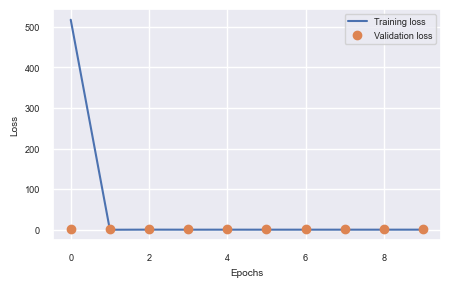
\includegraphics[width=0.7\textwidth]{loss_vs_epochs.png}
\caption{\label{fig:loss_vs_epochs}Comparison between validation loss before and after bias adjustment}
\end{figure}

\subsubsection{Model Training}

After fixing the default bias, the model training stage could be fully started with 100 epochs while the precision-recall curve (PRC) of validation data set was being monitored. 

\begin{lstlisting}[language=Python]
ann_model = make_model()
ann_model.load_weights(initial_weights)

baseline_history = ann_model.fit(
    train_features,
    train_labels,
    batch_size=BATCH_SIZE,
    epochs=EPOCHS,
    callbacks=[early_stopping],
    validation_data=(val_features, val_labels))
\end{lstlisting}

Also, the training history was recorded to verify over-fitting and to collect data for visualise some relevant metrics in this project, as they can be seen on Figure \ref{fig:ann_metrics}. The code used to plot the metrics is below:

\begin{lstlisting}[language=Python]
def plot_metrics(history):
    metrics = ['loss', 'prc', 'precision', 'recall']
    
    for n, metric in enumerate(metrics):
        name = metric.replace("_"," ").capitalize()
        plt.subplot(2,2,n+1)
        plt.plot(history.epoch, history.history[metric], color=colors[0], label='Train')
        plt.plot(history.epoch, history.history['val_' + metric],
                 color=colors[0], linestyle="--", label='Val')
        plt.xlabel('Epoch')
        plt.ylabel(name)
        
        if metric == 'loss':
            plt.ylim([0, plt.ylim()[1]])
        else:
            plt.ylim([0,1])

        plt.legend()

plot_metrics(baseline_history)
\end{lstlisting}

Ultimately, the training process was interrupted by the resource \emph{EarlyStopping} after 58 epochs after not registering a better PRC for 10 epochs. More details about the metrics were presented at Evaluation section of this work.

\begin{figure}
\centering
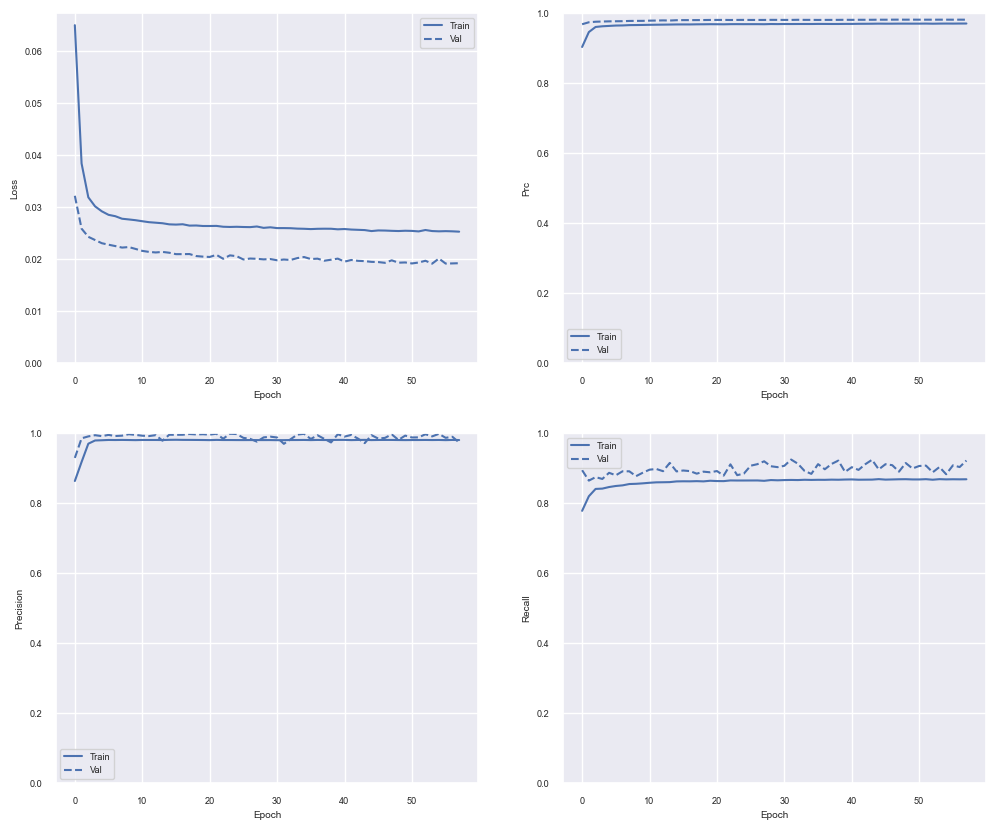
\includegraphics[width=1\textwidth]{ann_metrics.png}
\caption{\label{fig:ann_metrics}Metrics History After 58 Epochs}
\end{figure}

\subsection{Decision Tree Classifier}
As the data is not linearly separable and it's not possible to find a condition of 100\% correctly classified by a hyperplane, a non-linear classifier is recommended, thus a Decision Tree Classifier was implemented as part of this benchmark. The code below retrieved a previously trained Decision Tree model which was persisted as a Pickle file, then it predicted the class labels for the features in \emph{X\_test}, and finally generated the respective Classification Report in comparison with the labels in \emph{y\_test}.

\begin{lstlisting}[language=Python]
with open(os.path.join('pickle', 'tree_pipeline.pkl'), 'rb') as f:     
    tree_pipeline = pickle.load(f)
    
y_predicted_tree = tree_pipeline.predict(X_test)

cr_tree = metrics.classification_report(y_test, y_predicted_tree, digits=5)
\end{lstlisting}

\subsubsection{Hyperparameter optimisation}
For finding the best parameters for this model, the hyperparameters to tune the model were specified. Then a pipeline was created with 1 step:
\begin{enumerate}
\item \emph{decisiontreeclassifier} which applies the Decision Tree model.
\end{enumerate}

Then, a grid search was performed using the above-mentioned pipeline and the hyperparameter grid to find the combination with the best accuracy metric with the default cross-validation, that is, a 5-fold cross-validation.
\begin{lstlisting}[language=Python]
from sklearn.tree import DecisionTreeClassifier

tree_pipeline = Pipeline([
    ('decisiontreeclassifier', DecisionTreeClassifier())
])

param_grid = {
    'decisiontreeclassifier__min_samples_split': [2, 5, 10],
    'decisiontreeclassifier__min_samples_leaf': [1, 2, 4],
    'decisiontreeclassifier__max_features': ['sqrt', 'log2']
}

grid_search_tree = GridSearchCV(
    tree_pipeline,
    param_grid=param_grid,
    n_jobs=-1,
    scoring='f1',
    verbose=1
)

grid_search_tree.fit(X_train, y_train)
\end{lstlisting}

After this, the one-step pipeline was redefined with the best parameters found considering the proposed scenario for consistency with other models:
\begin{enumerate}    
    \item DecisionTreeClassifier(max\_features='sqrt')
\end{enumerate}

\subsubsection{Model training}
Then the model was trained using a similar pipeline, but this time with the optimal combination of parameters.

\begin{lstlisting}[language=Python]
tree_pipeline = Pipeline([
    ('decisiontreeclassifier', DecisionTreeClassifier(
        min_samples_split=grid_search_tree.best_params_['decisiontreeclassifier__min_samples_split'],
        min_samples_leaf=grid_search_tree.best_params_['decisiontreeclassifier__min_samples_leaf'],
        max_features=grid_search_tree.best_params_['decisiontreeclassifier__max_features']
    ))
])

tree_pipeline.fit(X_train, y_train)
\end{lstlisting}

Although the training and the fitting for this model was one of the the least sophisticated among all 5 models, the resulting decision tree was too complex to be visualised with details in this project. However, an overview of this tree can be seen on Figure \ref{fig:decision_tree}.

\begin{figure}
\centering

\includegraphics[width=1\textwidth]{decision_tree.png}
\caption{\label{fig:decision_tree}Overview of the Decision Tree Classifier for 3W Data Set}
\end{figure}

\subsection{Random Forest Classifier} 
As the data is not linearly separable and it's not possible to find a condition of 100\% correctly classified by a hyperplane, a non-linear classifier is recommended, thus a Random Forest Classifier was implemented as part of this benchmark. The following code loaded a previously trained Random Forest Classifier model which was saved as a Pickle file, then it predicted the class labels for the features in \emph{X\_test}, and finally generated the respective Classification Report in comparison with the labels in \emph{y\_test}.

\begin{lstlisting}[language=python]
with open(os.path.join('pickle', 'rf_pipeline.pkl'), 'rb') as f:    
rf_pipeline = pickle.load(f)
    
y_predicted_rf = rf_pipeline.predict(X_test)

cr_rf = metrics.classification_report(y_test, y_predicted_rf, digits=5)
\end{lstlisting}

\subsubsection{Hyperparameter optimisation}
For finding the best parameters for this model, the hyperparameters to tune the model were specified. Then a pipeline was created with 1 step:
\begin{enumerate}
\item \emph{randomforestclassifier} which applies the Random Forest model.
\end{enumerate}

Then, a grid search was performed using the above-mentioned pipeline and the hyperparameter grid to find the combination with the best accuracy metric with the default cross-validation, that is, a 5-fold cross-validation. Similar to \emph{LinearSVC}, the parameter \emph{class\_weight} was listing 2 possible values, \emph{balanced} and \emph{balanced\_subsample}, during hyperparametrisation tuning. The former also adjusts the weights in the same way as previously described, while the latter works similarly, except that weights are computed based on the bootstrap sample for every tree grown.


\begin{lstlisting}[language=Python]
from sklearn.ensemble import RandomForestClassifier

rf_pipeline = Pipeline([
    ('randomforestclassifier', RandomForestClassifier())
])

param_grid = {
    'randomforestclassifier__class_weight': ['balanced', 'balanced_subsample']
}

grid_search_rf = GridSearchCV(
    rf_pipeline,
    param_grid=param_grid,
    n_jobs=-1,
    scoring='f1',
    verbose=1
)

grid_search_rf.fit(X_train, y_train)
\end{lstlisting}

Then, the one-step pipeline was redefined with the best parameter found considering the proposed scenario:
\begin{enumerate}    
    \item RandomForestClassifier(class\_weight='balanced')
\end{enumerate}

\subsubsection{Model training}
Then the model was trained using a similar pipeline, but this time with the optimal combination of parameters.

\begin{lstlisting}[language=Python]
rf_pipeline = Pipeline([
    ('randomforestclassifier', RandomForestClassifier(
        class_weight=grid_search_rf.best_params_['randomforestclassifier__class_weight']
    ))
])

rf_pipeline.fit(X_train, y_train)
\end{lstlisting}

\section{Evaluation}

\subsection{Classification Report}

As it could be seen in Modeling section, the classification reports for all models were generated immediately after they were instantiated and they were all detailed in this section.

\subsubsection{LinearSVC}
\begin{lstlisting}[language=Python]
# printing classification report for LinearSVC
print(cr_linearsvc)
\end{lstlisting}
\begin{verbatim}  
              precision    recall  f1-score   support

           0     0.9980    0.9808    0.9893   2763432
           1     0.7568    0.9687    0.8498    170839

    accuracy                         0.9801   2934271
   macro avg     0.8774    0.9747    0.9195   2934271
weighted avg     0.9840    0.9801    0.9812   2934271
\end{verbatim}

\subsubsection{k-Neighbors Classifier}
\begin{lstlisting}[language=Python]
# printing classification report for kNN classifier
print(cr_knn)
\end{lstlisting}
\begin{verbatim}  
              precision    recall  f1-score   support

           0    0.99987   0.99487   0.99736   2763432
           1    0.92328   0.99787   0.95913    170839

    accuracy                        0.99505   2934271
   macro avg    0.96157   0.99637   0.97825   2934271
weighted avg    0.99541   0.99505   0.99514   2934271
\end{verbatim}

\subsubsection{Neural Networks}
\begin{lstlisting}[language=Python]
# printing classification report for ANN
print(cr_ann)
\end{lstlisting}
\begin{verbatim}    
              precision    recall  f1-score   support

           0    0.99321   0.99987   0.99653   2763432
           1    0.99760   0.88938   0.94039    170839

    accuracy                        0.99343   2934271
   macro avg    0.99541   0.94462   0.96846   2934271
weighted avg    0.99346   0.99343   0.99326   2934271
\end{verbatim}

\subsubsection{Decision Tree}
\begin{lstlisting}[language=Python]
# printing classification report for Decision Tree
print(cr_tree)
\end{lstlisting}
\begin{verbatim}
              precision    recall  f1-score   support

           0    0.99999   0.99972   0.99986   2763432
           1    0.99553   0.99980   0.99766    170839

    accuracy                        0.99973   2934271
   macro avg    0.99776   0.99976   0.99876   2934271
weighted avg    0.99973   0.99973   0.99973   2934271
\end{verbatim}

\subsubsection{Random Forest}
\begin{lstlisting}[language=Python]
# printing classification report for Random Forest
print(cr_rf)
\end{lstlisting}
\begin{verbatim}   
              precision    recall  f1-score   support

           0    1.00000   0.99991   0.99995   2763432
           1    0.99852   1.00000   0.99926    170839

    accuracy                        0.99991   2934271
   macro avg    0.99926   0.99995   0.99961   2934271
weighted avg    0.99991   0.99991   0.99991   2934271

\end{verbatim}


\subsection{Confusion Matrices}
In this section the confusion matrices for every model for test labels were computed and plotted side by side on Figure \ref{fig:confusion_matrices}.

\begin{figure}
\centering
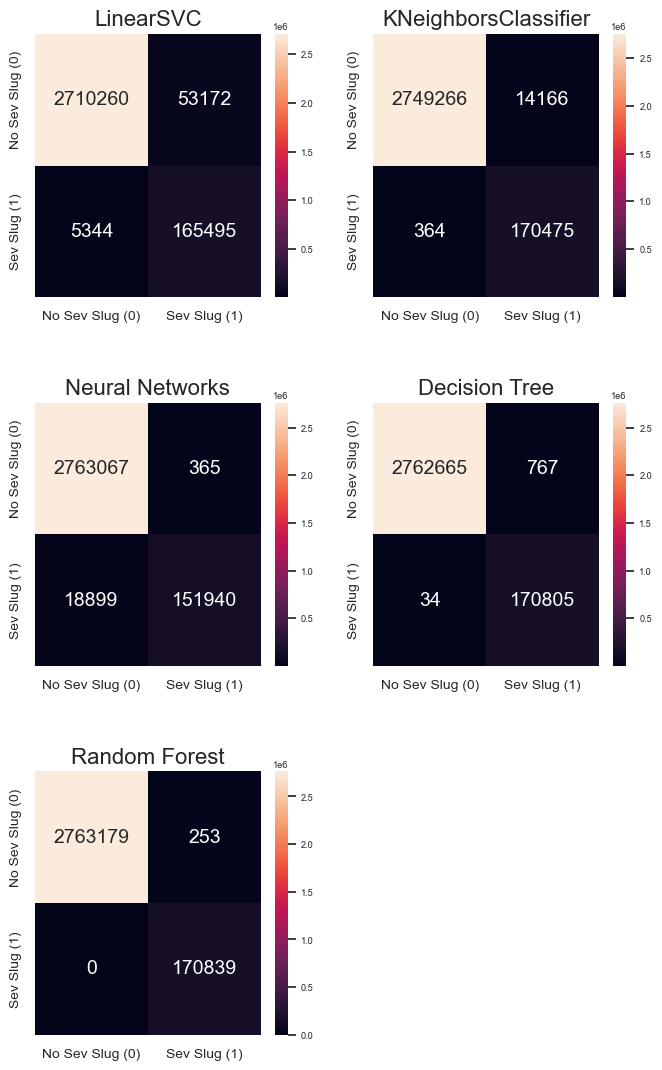
\includegraphics[width=0.75\textwidth]{confusion_matrices.png}
\caption{\label{fig:confusion_matrices}Confusion matrices showing the performance of five machine learning models in predicting severe slugging occurrences}
\end{figure}

\subsection{10-Fold Cross Validation}
Lastly, a K-Folds cross-validator was selected to split training data set into 10 consecutive folds and compute the mean accuracy and the respective standard deviation for each model. Computing this report with TensorFlow 2.0 and Keras demanded a particular implementation, given the inputs requested by the function which instantiates this model in this project. Moreover, this cross-validation report had to be compatible and conceptually comparable to the reports ordinarily generated by the method \emph{cross\_val\_score)}, that is, it should have the same information and data structure. 

Consequently, a customised 10-fold cross-validation implementation for ANN was built in the following code, which was adapted from a solution proposed by \textcite{christianversloot_2022}

\begin{lstlisting}[language=Python]
# implementing 10-fold cross-validation for NN

number_folds = 10
kfold = KFold(n_splits=number_folds, shuffle=True, random_state=42)

acc_per_fold = prec_per_fold = rec_per_fold = loss_per_fold = []

# Merge inputs and targets. 
# At this point features and labels must be already scaled
inputs = np.concatenate((train_features, test_features), axis=0)
targets = np.concatenate((train_labels, test_labels), axis=0)

number_epochs = 58

fold_no = 1

print('#' * 72)
for train, test in kfold.split(inputs, targets):
    model = make_model()

    # Generate a print
    print(f'Fold #{fold_no}...')

    # Fit data to model
    history = model.fit(
      inputs[train], targets[train],
      batch_size=BATCH_SIZE,
      epochs=number_epochs,
      verbose=1
    )

    # Generate generalization metrics
    scores = model.evaluate(inputs[test], targets[test], batch_size=BATCH_SIZE, verbose=0)
    
    print(f'\nScores for Fold #{fold_no}:') 
    
    fold_loss = (model.metrics_names[0], scores[0])
    fold_accu = (model.metrics_names[5], scores[5])
    fold_prec = (model.metrics_names[6], scores[6])
    fold_recl = (model.metrics_names[7], scores[7])
    
    print(f'{fold_loss[0]} = {fold_loss[1]};')
    print(f'{fold_accu[0]} = {fold_accu[1]};')
    print(f'{fold_prec[0]} = {fold_prec[1]};')
    print(f'{fold_recl[0]} = {fold_recl[1]};')

    loss_per_fold.append(fold_loss[1])
    acc_per_fold.append(fold_accu[1])
    prec_per_fold.append(fold_prec[1])
    rec_per_fold.append(fold_recl[1])

    fold_no = fold_no + 1
\end{lstlisting}

The other models were still put on the same pipelines used on modeling section.

\begin{lstlisting}[language=Python]
models = [    
    ('Decision Tree', tree_pipeline),
    ('Linear SVC', linear_svc_pipeline),
    ('KNeighborsClassifier', knn_pipeline),    
    ('Random Forest', rf_pipeline)
]
\end{lstlisting}

After an empty dictionary to host the results from the cross-validation was initialised, a 10-fold cross-validation for each model (except ANN) was computed for 3 metrics, namely: accuracy, precision and recall.

\begin{lstlisting}[language=Python]
cross_validation_dict = dict()

cv_metrics = ['accuracy','precision','recall']

cross_validation_dict = {name: {} for name, _ in models}

for cv_metric in cv_metrics:
    print(f'\nStarting a {number_folds}-fold CV for {cv_metric}...')
    for name, model in models:
        cv_results = cross_val_score(model, X_train, y_train, cv=kfold, scoring=cv_metric)
        cross_validation_dict[name][cv_metric] = cv_results
        msg = "-> %s: %f (%f)" % (name, np.nanmean(cv_results), np.nanstd(cv_results))        
        print(msg)   
\end{lstlisting}
\begin{verbatim}
Starting a 10-fold CV for accuracy...
-> Decision Tree: 0.999781 (0.000063)
-> Linear SVC: 0.974574 (0.000481)
-> KNeighborsClassifier: 0.996025 (0.000240)
-> Random Forest: 0.999948 (0.000022)

Starting a 10-fold CV for precision...
-> Decision Tree: 0.999718 (0.000098)
-> Linear SVC: 0.980681 (0.000688)
-> KNeighborsClassifier: 0.994433 (0.000448)
-> Random Forest: 0.999902 (0.000047)

Starting a 10-fold CV for recall...
-> Decision Tree: 0.999844 (0.000089)
-> Linear SVC: 0.968222 (0.000686)
-> KNeighborsClassifier: 0.997635 (0.000242)
-> Random Forest: 0.999995 (0.000010)
\end{verbatim}

After this, the cross-validation results computed for ANN were added to the cross-validation dictionary.

\begin{lstlisting}
cv_val_dict = cross_validation_dict

cv_val_dict['Neural Networks'] = dict()
cv_val_dict['Neural Networks']['accuracy'] = np.array(acc_per_fold)
cv_val_dict['Neural Networks']['precision'] = np.array(prec_per_fold)
cv_val_dict['Neural Networks']['recall'] = np.array(rec_per_fold)    

models.append(('Neural Networks', False))
\end{lstlisting}

The following code was implemented to plot how each metric averaged in each model. These corresponding charts can be visualised on Figures \ref{fig:10_fold_acc}, \ref{fig:10_fold_prec} and \ref{fig:10_fold_rec}.

\begin{lstlisting}[language=Python]
def plot_metric_boxplot(metric, cv_val_dict, number_folds):
    data = [cv_val_dict[model][metric] for model in cv_val_dict.keys()]
    fig = plt.figure()
    fig.suptitle(f'Distribution of Mean {metric.capitalize()} After {number_folds}-Fold Cross Validation By Algorithm')
    ax = fig.add_subplot(111)
    plt.boxplot(data)
    ax.set_xticklabels(cv_val_dict.keys())
    fig.set_size_inches(8,4)
    plt.show()

plot_metric_boxplot('accuracy', cv_val_dict, number_folds)
plot_metric_boxplot('precision', cv_val_dict, number_folds)
plot_metric_boxplot('recall', cv_val_dict, number_folds)
\end{lstlisting}

\begin{figure}
\centering
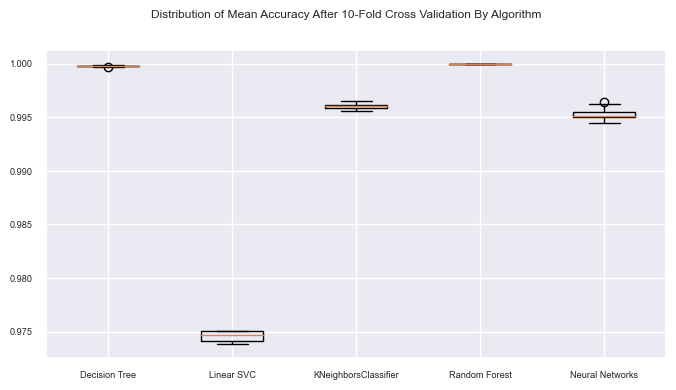
\includegraphics[width=0.75\textwidth]{10_fold_acc.png}
\caption{\label{fig:10_fold_acc}Box plots showing the distribution of Mean Accuracy After 10-fold Cross Validation By Algorithm}
\end{figure}.

\begin{figure}
\centering
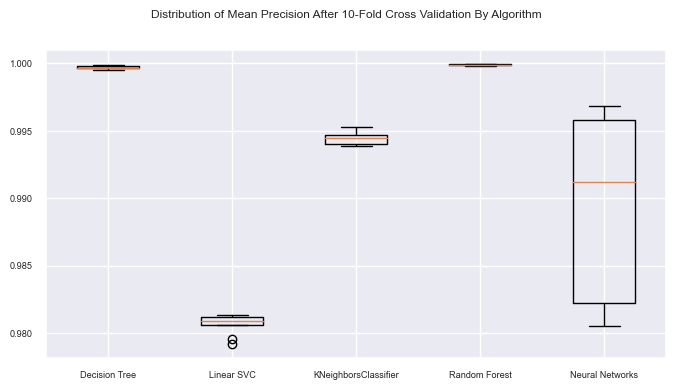
\includegraphics[width=0.75\textwidth]{10_fold_prec.png}
\caption{\label{fig:10_fold_prec}Box plots showing the distribution of Mean Accuracy After 10-fold Cross Validation By Algorithm}
\end{figure}.

\begin{figure}
\centering
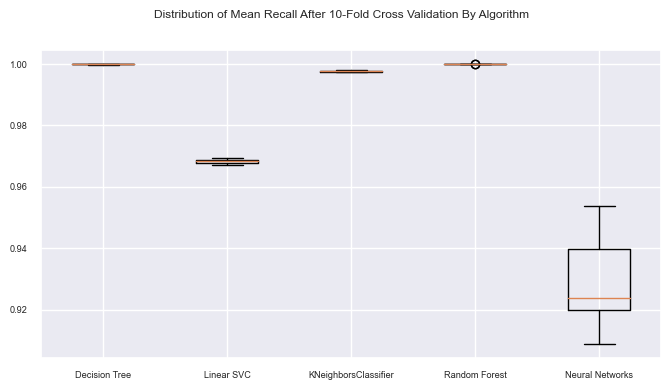
\includegraphics[width=0.75\textwidth]{10_fold_rec.png}
\caption{\label{fig:10_fold_rec}Box plots showing the distribution of Mean Accuracy After 10-fold Cross Validation By Algorithm}
\end{figure}.


\section{Conclusion}

The general goal of this capstone work was developing and using machine learning approaches to detect the presence and the absence of Severe Slugging in an offshore well production line, considering as a reference the real instances from 3W data set. In addition to this, after the definition of three metrics as success criteria (accuracy, precision and recall) and the definition of a baseline score, an eligible classification model must present significant results in all 3 metrics. 

This work managed to find 2 models with satisfactory results in all selected metrics, namely Random Forest Classifier and Decision Tree Classifier. This was possible due to:
\begin{enumerate}
    \item Adopting CRISP-DM, which enabled the group to correctly plan a hypothesis, build a minimally viable implementation, measuring the results and making the necessary adjustments before proceeding to another iteration; 
    \item Understanding the business domain, the data set and then selecting the most promising features, after identifying the strongest correlations between them and the target;    
    \item Defining the data had no clear linear separability, by visualising the results from dimensionality reduction with 2 and 3 components and by measuring the score from a LinearSVC model, which enabled this project to invest more resources on non-linear classifiers;
    \item Implementing solutions to assertively evaluate the results in all 5 models according the selected metrics
\end{enumerate}

Overall, the results presented here show the potential for classification models to enhance the detection of Severe Slugging. Once such models are deployed, they may help an offshore oil operation to mitigate operational and environmental risks, reduce costs in operation and improve the production efficiency, as it could mitigate operational losses. Also, the methods and techniques used in this project can be further improved and extended to detect other undesirable events not only in 3W Data Set but also in the general oil and gas industry.

\iffalse

% \subsection{How to write Mathematics}

% \LaTeX{} is great at typesetting mathematics. Let $X_1, X_2, \ldots, X_n$ be a sequence of independent and identically distributed random variables with $\text{E}[X_i] = \mu$ and $\text{Var}[X_i] = \sigma^2 < \infty$, and let
% \[S_n = \frac{X_1 + X_2 + \cdots + X_n}{n}
%       = \frac{1}{n}\sum_{i}^{n} X_i\]
%  denote their mean. Then as $n$ approaches infinity, the random variables $\sqrt{n}(S_n - \mu)$ converge in distribution to a normal $\mathcal{N}(0, \sigma^2)$.


\fi

\printbibliography

\end{document}